\documentclass[12pt]{article}

\usepackage{amssymb,amsmath,amsthm}
\usepackage[top=1in, bottom=1in, left=1.25in, right=1.25in]{geometry}
\usepackage{fancyhdr}
\usepackage{enumerate}
\usepackage[bw,framed,numbered]{mcode}
\usepackage{graphicx}

% Comment the following line to use TeX's default font of Computer Modern.
\usepackage{times,txfonts}

\newtheoremstyle{homework}% name of the style to be used
  {18pt}% measure of space to leave above the theorem. E.g.: 3pt
  {12pt}% measure of space to leave below the theorem. E.g.: 3pt
  {}% name of font to use in the body of the theorem
  {}% measure of space to indent
  {\bfseries}% name of head font
  {:}% punctuation between head and body
  {2ex}% space after theorem head; " " = normal interword space
  {}% Manually specify head
\theoremstyle{homework} 

% Set up an Exercise environment and a Solution label.
\newtheorem*{exercisecore}{Exercise \@currentlabel}
\newenvironment{exercise}[1]
{\def\@currentlabel{#1}\exercisecore}
{\endexercisecore}

\newcommand{\localhead}[1]{\par\smallskip\noindent\textbf{#1}\nobreak\\}%
\newcommand\solution{\localhead{Solution:}}

%%%%%%%%%%%%%%%%%%%%%%%%%%%%%%%%%%%%%%%%%%%%%%%%%%%%%%%%%%%%%%%%%%%%%%%%
%
% Stuff for getting the name/document date/title across the header
\makeatletter
\RequirePackage{fancyhdr}
\pagestyle{fancy}
\fancyfoot[C]{\ifnum \value{page} > 1\relax\thepage\fi}
\fancyhead[L]{\ifx\@doclabel\@empty\else\@doclabel\fi}
\fancyhead[C]{\ifx\@docdate\@empty\else\@docdate\fi}
\fancyhead[R]{\ifx\@docauthor\@empty\else\@docauthor\fi}
\headheight 15pt

\def\doclabel#1{\gdef\@doclabel{#1}}
\doclabel{Use {\tt\textbackslash doclabel\{MY LABEL\}}.}
\def\docdate#1{\gdef\@docdate{#1}}
\docdate{Use {\tt\textbackslash docdate\{MY DATE\}}.}
\def\docauthor#1{\gdef\@docauthor{#1}}
\docauthor{Use {\tt\textbackslash docauthor\{MY NAME\}}.}
\makeatother

% Shortcuts for blackboard bold number sets (reals, integers, etc.)
\newcommand{\Reals}{\ensuremath{\mathbb R}}
\newcommand{\Nats}{\ensuremath{\mathbb N}}
\newcommand{\Ints}{\ensuremath{\mathbb Z}}
\newcommand{\Rats}{\ensuremath{\mathbb Q}}
\newcommand{\Cplx}{\ensuremath{\mathbb C}}
%% Some equivalents that some people may prefer.
\let\RR\Reals
\let\NN\Nats
\let\II\Ints
\let\CC\Cplx

%%%%%%%%%%%%%%%%%%%%%%%%%%%%%%%%%%%%%%%%%%%%%%%%%%%%%%%%%%%%%%%%%%%%%%%%%%%%%%%%%%%%%%%
%%%%%%%%%%%%%%%%%%%%%%%%%%%%%%%%%%%%%%%%%%%%%%%%%%%%%%%%%%%%%%%%%%%%%%%%%%%%%%%%%%%%%%%
% 
% The main document start here.

% The following commands set up the material that appears in the header.

%%%%%%%%%%%%%%%%%%%%%%%%%%%%%%%%%%%%%%%%%%%%%%%%%%%%%%%%%%%%%%%%%%%%%%%%%%%%%%%%%%%%%%%
%%%%%%%%%%%%%%%%%%%%%%%%%%%%%%%%%%%%%%%%%%%%%%%%%%%%%%%%%%%%%%%%%%%%%%%%%%%%%%%%%%%%%%%
% 
% The main document start here.

% The following commands set up the material that appears in the header.
\doclabel{Math 310: Homework 3}
\docauthor{Parker Whaley}
\docdate{August 22, 2016}

\newcommand{\vv}{\mathbf{v}}
\begin{document}
\begin{exercise}

Write down the 4th order Taylor polynomial of $\sqrt{
x}$ centered at $x = 1$. Let $P(x)$ denote
this polynomial. If $1 \leq x \leq 2$, what can you say about the size of $|\sqrt{x} - P(x)|$? Hint: Use
the remainder term!
\end{exercise}
Lets start by getting the derivatives of $f(x)=\sqrt{x}$.
$$f(x)=x^\frac{1}{2}$$
$$f'(x)=\frac{1}{2}x^{-\frac{1}{2}}$$
$$f''(x)=-\frac{1}{4}x^{-\frac{3}{2}}$$
$$f'''(x)=\frac{3}{8}x^{-\frac{5}{2}}$$
$$f^{(4)}(x)=-\frac{15}{16}x^{-\frac{7}{2}}$$
$$f^{(5)}(x)=\frac{105}{32}x^{-\frac{9}{2}}$$

Now we can construct $P(x)$ as 
$$P(x)=1^\frac{1}{2}+\frac{1}{2}1^{-\frac{1}{2}}(x-1)+-\frac{1}{2}\frac{1}{4}1^{-\frac{3}{2}}(x-1)^2+\frac{1}{6}\frac{3}{8}1^{-\frac{5}{2}}(x-1)^3+-\frac{1}{24}\frac{15}{16}1^{-\frac{7}{2}}(x-1)^4$$
$$P(x)=1+\frac{1}{2}(x-1)-\frac{1}{8}(x-1)^2+\frac{1}{16}(x-1)^3-\frac{5}{128}(x-1)^4$$
Note that the remainder term would be
$$R(x)=\frac{1}{5!}\frac{105}{32}\xi^{-\frac{9}{2}}(x-1)^5=\frac{7}{256}\xi^{-\frac{9}{2}}(x-1)^5$$
Where $f(x)=P(x)+R(x)$.
We are now asked to compute the error, $E$, in the case that $1 \leq x \leq 2$. We see that $E=|f(x) - P(x)|=|R(x)|=|\frac{7}{256}\xi^{-\frac{9}{2}}(x-1)^5|$ and noting that $\xi,x\in [1,2]$ we get $E=\frac{7}{256}\xi^{-\frac{9}{2}}(x-1)^5$.  The maximum value E could have would be $x=2$ and $\xi=1$ so $E_{max}=\frac{7}{256}$ and of course the smallest value is at $x=1$ where by our construction $f(x)=p(x)$ so $0\leq E\leq \frac{7}{256}$.
\newpage
\begin{exercise}

Chapter 4: 2 (b)
\end{exercise}
This is my code for newton's method.
\lstinputlisting{../octave/newton.m}
\newpage
And this is my driver for newton's method
\lstinputlisting{../octave/question_2b.m}
\newpage
\lstinputlisting{../octave/diy_q2b.txt}
Noting that the expected errors and the actual errors appear to be very similar I conclude that the method for estimating error in y is valid and conclude that it will take one more iteration to have a error less than $10^-16$.
\begin{exercise}

Chapter 4: 3
\end{exercise}
Estimating $\frac{1}{3}$ by newtons method.
$$f=x^{-1}-3$$
$$f'=-x^{-2}$$
$$x_{k+1}=x_k+\frac{x_k^{-1}-3}{x_k^{-2}}
=x_k+x_k-3x_k^2
=2x_k-3x_k^2$$
Now using $x_0=.5$ I can calculate an estimate for $\frac{1}{3}$.
$$x_0=.5$$
$$x_1=.25$$
$$x_2=.3125$$
$$x_3=.3203$$
$$x_4=.3333$$
This method definitely approaches the true value of $\frac{1}{3}$.\\
Lets try again with $x_0=1$
$$x_0=1$$
$$x_1=-1$$
$$x_2=-5$$
$$x_3=-85$$
Clearly not approaching $\frac{1}{3}$.\\
\begin{exercise}

Chapter 4: 4
\end{exercise}
Note that $f(x)=x^2-2$ has a root at $x=\sqrt{2},-\sqrt{2}$.  So if we do newtons method we should find a approximation for $\sqrt{2}$.
\lstinputlisting{../octave/q4.txt}

\begin{exercise}

Chapter 4: 6
\end{exercise}
\begin{enumerate}[(a)]

\item
Assuming $h(x)$ is differentiable, witch by inspection in this case it is, all extrema occur at zeros of $h'(x)=x^3-3$.  Noting that $h''(x)=3x^2$ we get newtons method as: $$x_{k+1}=x_k-\frac{x_k^3-3}{3x_k^2}$$

\item
Taking one newtons method step with $x_0=1$ I get:
$$x_{2}=1-\frac{1-3}{3}=1+2/3\approx 1.66$$

\item
First note that $h'(0)=-3$ and $h'(4)>0$, now we know where to replace negative and positive values.  Now the midpoint value would be $h'(2)=5$, so our new interval would be $[0,2]$.  The midpoint value of these two would be $h'(1)=-2$.  So after two midpoint steps our interval would be $[1,2]$.

\end{enumerate}

\begin{exercise}

Chapter 4: 9
\end{exercise}
\begin{enumerate}[(a)]
\item
The bisection method is not usable in this case. For the bisection method we need to start with two $x$ values one of witch has a negative $f(x)$ and one that has a positive $f(x)$.  The function $f(x)=\sin (x)+1$ is never negative, thus we can't choose two points to use the bisection method on.

\item
Newtons method will work however since at any point where $f(x)=0$ we know that $f'(x)=0$ the method should not approach quadratically but only linearly.
\end{enumerate}

\begin{exercise}

Chapter 4: 10
\end{exercise}
running the bisect method
\lstinputlisting{../octave/q10.m}
\lstinputlisting{../octave/q10.txt}
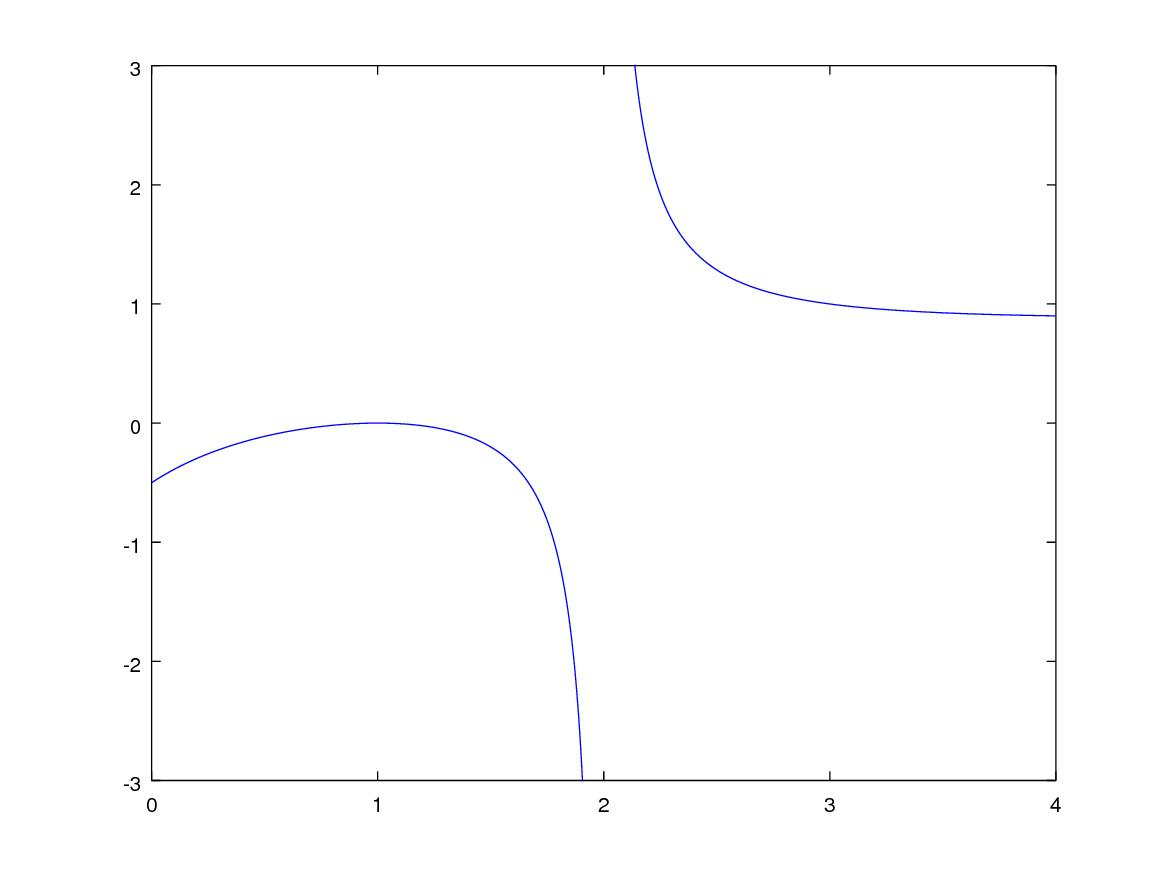
\includegraphics[scale=.4]{../octave/q20fig.jpg}\\
This method is clearly not going to the root.  This is because the bisect method goes to the place where $f(x)$ changes sign, in this case that would be the asimtote at $x=2$.  In the range $[0,1.5]$ the intermediate value therm does not guarantee a root since both $0$ and $1.5$ have negative associated $f(x)$ values.  In the range $[1.5,3]$ the intermediate value therm does not guarantee a root since $f(x)$ has a discontinuity at $x=2$.

\begin{exercise}

Chapter 4: 11
\end{exercise}
\begin{enumerate}[(a)]
\item
$f(x)=\sin (x)$, $f'(x)=\cos (x)$
$$x_{k+1}=x_k-\frac{\sin (x_k)}{\cos (x_k)}$$
NB  This newton's method gives us $\pi$ but the evaluation of $\sin$ internally may use $\pi$, so I wouldn't necessarily think this is a way to find the value of $\pi$.

\item
$f(x)=x^3-x^2-2x$, $f'(x)=3x^2-2x-2$
$$x_{k+1}=x_k-\frac{x_k^3-x_k^2-2x_k}{3x_k^2-2x_k-2}$$

\item
$f(x)=1-.01x$, $f'(x)=-.01$
$$x_{k+1}=x_k-\frac{1-.01x}{-.01}$$
In this case one step of newtons method should get us to the exact root.  Newtons method estimates a curve by a line that has the same slope and value as the curve at some point $x_k$ then uses the root of that line as a guess of the root of the curve.  Since in this case the curve is a line newtons idea to estimate it as a line is exact and one run of newtons method, regardless of starting position will take us to the answer.
\end{enumerate}
\lstinputlisting{../octave/q11.m}
\newpage
\lstinputlisting{../octave/q11.txt}
\end{document}